%% Exemple de source LaTeX pour un article soumis à TALN
\documentclass[10pt,a4paper,twoside]{article}

\usepackage[greek,frenchb,english]{babel}
%\usepackage{times}
\usepackage{mathptmx}           %%%%%%%%%%%%%%%%
\usepackage[scaled=.92]{helvet} % police Times %
\usepackage{courier}            %%%%%%%%%%%%%%%%
\usepackage[utf8x]{inputenc}
\usepackage[T1]{fontenc}
\usepackage{graphicx}

\usepackage{url}
\usepackage[dvipsnames,svgnames]{xcolor}
\usepackage{footnote}
\makesavenoteenv{tabular}
\usepackage{natbib}
%\makesavenoteenv{tabular}
% faire les \usepackage dont vous avez besoin avant le \usepackage{taln2010} 

\usepackage{taln2011}
%\usepackage[frenchb]{babel}
\def\textgreek#1{\leavevmode{\fontfamily{cmr}\greektext #1}}

\title{Détection de zones parallèles à l'intérieur de bi-documents}

\author{Charlotte Lecluze\up{1, 2}\quad Romain Brixtel\up{1}\\
  (1) GREYC, Université de Caen Basse-Normandie, France\\ 
  (2) Pertimm, Asnières-sur-Seine, France \\ 
  prénom.nom@\{unicaen.fr, pertimm.com\}\\ 
}

\fancyhead[CO]{Détection de zones parallèles à l'intérieur de bi-documents} 
\fancyhead[CE]{Charlotte Lecluze, Romain Brixtel} 

\begin{document}

\maketitle

\resume{
Dans cet article, nous présentons un des principaux axes de nos travaux en matière d'alignement multilingue et endogène de multidocuments. La question que nous abordons ici est celle du parallélisme entre les différents \textit{volets} d'un bi-document. Loin de présupposer un parallélisme global entre ces volets, nous proposons une méthode endogène pour définir en contexte les zones qui maximisent le parallélisme : documents, séquences de paragraphes, paragraphes,... Cette étape repose sur un appariement de N-grammes de caractères répétés et constitue une étape préalable à un alignement lexical.
}

\abstract{In this paper, we present one of the main axes of our work in progress concerning multilingual and endogenous alignment of multidocuments. The question that we address here is the one of the parallelism between the different components of a bi-document. Far from presupposing a global parallelism between these components, we propose a endogenous method for defining in context the areas that maximize the parallelism: documents, sequences of paragraphs, paragraphs, ... This step is based on a matching of repeated character N-grams and is a preliminary step to a lexical alignment.
}

\motsClefs{détection et alignement de zones, appariement de N-grammes de caractères, collection de multidocuments}
{area detection and alignment, character N-grams matching, set of multidocuments}

%% Aller à la page suivante si nécessaire
%\newpage
%%================================================================
\section{Introduction}
L'opération traduisante, réalisée par l'humain et visant à traduire un document donné dans une langue source dans une langue cible, donne lieu à de nombreuses modifications dans l'organisation interne des différents \textit{volets} ou versions d'un multidocument tant au niveau micro qu'au niveau macro. Cette possibilité que l'ordre macro ne soit pas globalement maintenu d'un \textit{volet} à un autre, par exemple lorsqu'un résumé présent au début d'un volet et à la fin d'un ou de plusieurs autres, ou encore en présence d'une liste triée par ordre alphabétique (cf. figure \ref{inversion.png}), constitue un des principaux obstacles aux méthodes d'alignement de documents.


% \begin{center}
%  \includegraphics[bb=0 0 877 601]{../../../../../../home/charlotte/Images/inversion.png}
%  % inversion.png: 877x601 pixel, 72dpi, 30.94x21.20 cm, bb=0 0 877 601
% \end{center}

\begin{figure}[!t]
  \begin{center}
  \setlength{\unitlength}{0.9cm}
\begin{picture}(16,10.5)
{\small
    \put(0,10.2){{\large {\bf Volet français}}}
    \put(0,9.5){Allemagne - six projets}
    \put(0,9){[...]}
    \put(0,8){Belgique - deux projets}
    \put(0,7.5){[...]}
    \put(0,6.5){Danemark - six projets}
    \put(0,6){[...]}
    \put(0,5){Espagne - seize projets}
    \put(0,4.5){[...]}
    \put(0,3.5){Estonie - un projet}
    \put(0,3){[...]}
    \put(0,2){Finlande - deux projets}
    \put(0,1.5){[...]}
    \put(0,0.5){Royaume-unis - dix projets}
    \put(0,0){[...]}

    \put(5.5,10.2){{\large {\bf Volet anglais}}}
    \put(5.5,9.5){Belgium - 2 projects}
    \put(5.5,9){[...]}
    \put(5.5,8){Denmark - 6 projects}
    \put(5.5,7.5){[...]}
    \put(5.5,6.5){Estonia - 1 project}
    \put(5.5,6){[...]}
    \put(5.5,5){Finland - 2 projects}
    \put(5.5,4.5){[...]}
    \put(5.5,3.5){Germany - 6 projects}
    \put(5.5,3){[...]}
    \put(5.5,2){Spain - 16 projects}
    \put(5.5,1.5){[...]}
    \put(5.5,0.5){United Kingdom - 10 projets}
    \put(5.5,0){[...]}

    \put(11,10.2){{\large {\bf Volet allemand}}}
    \put(11,9.5){Belgien - zwei Projekte}
    \put(11,9){[...]}
    \put(11,8){Dänemark - sechs Projekte}
    \put(11,7.5){[...]}
    \put(11,6.5){Estland - ein Projekte}
    \put(11,6){[...]}
    \put(11,5){Finnland - swei Projekte}
    \put(11,4.5){[...]}
    \put(11,3.5){Deutschland - sechs Projekte}
    \put(11,3){[...]}
    \put(11,2){Spanien - 16 Projekte}
    \put(11,1.5){[...]}
    \put(11,0.5){Vereinigtes Königreich - zehn Projekte}
    \put(11,0){[...]}


    \put(4.2,9.6){\circle*{0.1}}
    \put(4.2,9.6){\line(1,-6){1}}
    \put(4.2,8.1){\circle*{0.1}}
    \put(4.2,8.1){\line(2,3){1}}
    \put(4.2,6.6){\circle*{0.1}}
    \put(4.2,6.6){\line(2,3){1}}
    \put(4.2,5.1){\circle*{0.1}}
    \put(4.2,5.1){\line(1,-3){1}}
    \put(4.2,3.6){\circle*{0.1}}
    \put(4.2,3.6){\line(1,3){1}}
    \put(4.2,2.1){\circle*{0.1}}
    \put(4.2,2.1){\line(1,3){1}}
    \put(4.2,0.6){\circle*{0.1}}
    \put(4.2,0.6){\line(1,0){1}}


    \put(5.2,9.6){\circle*{0.1}}
    \put(5.2,8.1){\circle*{0.1}}
    \put(5.2,6.6){\circle*{0.1}}
    \put(5.2,5.1){\circle*{0.1}}
    \put(5.2,3.6){\circle*{0.1}}
    \put(5.2,2.1){\circle*{0.1}}
    \put(5.2,0.6){\circle*{0.1}}


    \put(9.7,9.6){\circle*{0.1}}
    \put(10.7,9.6){\circle*{0.1}}
    \put(9.7,9.6){\line(1,0){1}}
    \put(9.7,8.1){\circle*{0.1}}
    \put(10.7,8.1){\circle*{0.1}}
    \put(9.7,8.1){\line(1,0){1}}
    \put(9.7,6.6){\circle*{0.1}}
    \put(10.7,6.6){\circle*{0.1}}
    \put(9.7,6.6){\line(1,0){1}}
    \put(9.7,5.1){\circle*{0.1}}
    \put(10.7,5.1){\circle*{0.1}}
    \put(9.7,5.1){\line(1,0){1}}
    \put(9.7,3.6){\circle*{0.1}}
    \put(10.7,3.6){\circle*{0.1}}
    \put(9.7,3.6){\line(1,0){1}}
    \put(9.7,2.1){\circle*{0.1}}
    \put(10.7,2.1){\circle*{0.1}}
    \put(9.7,2.1){\line(1,0){1}}
    \put(9.7,0.6){\circle*{0.1}}
    \put(10.7,0.6){\circle*{0.1}}
    \put(9.7,0.6){\line(1,0){1}}



%    \put(1.9,0.3){\line(1,4){0.4}}
%    \put(5.7,0.3){\line(1,4){0.4}}

%    \put(9.8,0.3){\line(5.4,3){2.7}}
%    \put(11.3,0.3){\line(5.4,3){2.7}}
%    \put(12.6,0.3){\line(5.4,3){2.7}}
%    \put(13.9,0.3){\line(-6.6,3){3.3}}

%    \put(1,0.70){\vector(1,0){6}}
%    \put(2,0.25){\emph{ordre linéaire du texte}}
%    \put(0,5){\vector(0,-1){4}}
%    \begin{rotate}{-90}
%    \put(-4.5,-0.5){\emph{compositionnalité}}
%    \end{rotate}
}
\end{picture}

%\includegraphics[height=14cm,width=16cm]{inversion.png}
%\DeclareGraphicsRule{ext}{pdf}{readfile}{command}
\caption{
  \label{inversion.png}
  Maintien de l'ordre et inversions entre les différents volets
  d'un multidocument (communiqué de presse IP/05/1157 de l'Union
  Européenne) en anglais, français et allemand contenant des paragraphes
  triés par ordre alphabétique. Nous utilisons les [\dots] pour
  symboliser le contenu d'un paragraphe, dont nous ne conservons ici
  que le début soit le nom du pays dont il traite.} 
\end{center}
\end{figure}
%Les méthodes reposant sur une hypothèse de parallélisme se heurtent à ce type de variations. 
Cet article présente un outil graphique de détection du parallélisme entre les volets, endogène et sans traitement préalable des multidocuments. Notre objectif est double : 
\begin{itemize}
\item définir si la traduction est globalement littérale entre deux volets ;
\item pour les cas où l'hypothèse de parallélisme ne s'avère pas globalement vérifiée, délimiter et aligner les zones entre les volets.  
\end{itemize}

Plusieurs courants existent dans le domaine de l'alignement. Ils se distinguent notamment par le grain qu'ils proposent d'analyser : phrases, paragraphes, documents, ... Nous consacrerons donc la section 2 à un rapide tour d'horizon des principales méthodes d'alignement proposées à ce jour, avec un intérêt particulier pour l'alignement de documents. Dans la section 3, nous présenterons les points d'ancrage que nous utilisons dans le cadre de notre méthode d'alignement de zones à l'intérieur de bi-documents à la fois endogène et indépendante des langues. Enfin, dans la section 4, nous exposerons les outils graphiques de détection de zones que nous avons mis en place. \\

\section{Contexte}

% Les méthodes d'alignement automatique proposées vont du tout statistique (Gale et Church, 199), à des méthodes hybrides, alliant tant des indices de longueurs, de fréquences, que des indices lexicaux (Langlais, 1997). Les recherches ont d'abord porté sur la mise en correspondance de phrases. Le problème est considéré résolu, moyennant des hypothèses fortes sur la structure des multidocuments comme le rappelle (Véronis, 2000) :
% l'ordre des phrases des différents volets est identique ou très proche 
% les différents volets connaissent peu de suppressions ou d'adjonctions 
% les alignements 1:1 sont très largement prépondérants et les rares alignements m:n sont limités à de petites
% valeurs de m et n (typiquement 2).
% Les résultats des aligneurs se dégradent en fait rapidement lorsque ces hypothèses ne sont pas vérifiées.
% La difficulté d'exploiter des phrases alignées ont conduit à l'émergence de méthodes alignant à un grain inférieur à celui de la phrase : mots (Gale, 1991), chunks (Zhou et al., 2004), propositions (Nakamura-Delloye, 2007).
% Les méthodes d'alignement sous-phrastiques, si diverses soient-elles, trouvent toutes leur limite dans le fait qu'elles présupposent la disponibilité de corpus préalablement alignés en phrases (Hansard,...). De tels corpus sont cependant peu nombreux.
% En revanche, l’accessibilité grandissante à des documents en différentes langues laisse envisager la pratique d’opérations de rétro-ingénierie massives et peu supervisées sur ces documents issus du travail du traducteur humain. Ces pratiques permettent d’extraire des informations linguistiques et des ressources lexicales pouvant être utiles tant aux traducteurs, qu’aux lexicographes, aux linguistes ou aux terminologues.
% 
% Pour pallier ce problème, les méthodes d'alignement ont classiquement recours à un alignement préalable en phrases, ou encore à des ressources lexicales fournissant des points d'ancrage (Nakamura-Delloye).
% 
% Dagan,1993 => pas d'ali préalable en phrases 
% Simard, brown => cognats

Les méthodes d'alignement sous-phrastiques appliquées à des phrases alignées, si diverses soient-elles, trouvent toutes leur limite dans le fait qu'elles présupposent la disponibilité de corpus préalablement alignés en phrases (Hansard,...). De tels corpus sont cependant peu nombreux.\\
En revanche, l’accessibilité grandissante à des documents en différentes langues est avérée et laisse réellement envisager la pratique d’opérations de rétro-ingénierie massives et peu supervisées sur ces documents issus du travail du traducteur humain. Ces pratiques permettent d’extraire des informations linguistiques et des ressources lexicales pouvant être utiles tant aux traducteurs, qu’aux lexicographes, aux linguistes ou aux terminologues.\\
Plusieurs méthodes d'alignement sous-phrastique à partir de documents non préalablement alignés en phrases ont été proposées. (\citealp{simard_using_1993,church_char_align:_1993,church_dotplot:_1993,dagan_robust_1993}), établissant un lien entre la similitude de graphie et la similitude de sens, proposent de s'appuyer sur les similitudes de chaînes de caractères. Néanmoins, si ces similitudes sont fréquentes entre les langues indo-européennes, elles s'avèrent plus rares et insuffisantes entre les langues indo-européennes et les langues asiatiques par exemple. (\citealp{fung_k-vec:_1994,fung_aligning_1994}) quant-à-lui, à travers les systèmes K-vec et DK-vec, a proposé une méthode d'alignement de documents basée sur une similitude de répartition de mots. Les systèmes reposant sur la similitude de répartition de mots se heurtent à la nature flexionnelle de certaines langues, certaines mots pouvant recouvrir plusieurs formes selon leur fonction dans la phrase.\\

Para sur les outils de détection graphique  Chang \citep{chang_alignment_1997}\\

Nos recherches nous ont menés à nous intéresser aux N-grammes de caractères répétés propices à révéler des similitudes à la fois monolingues et multilingues susceptibles de nous aider dans la détection de zones maximisant le parallélisme entre les volets d'un bi-document. Grâce à eux, nous réalisons un alignement grossier des volets de bi-documents à partir d'une collection de bi-documents.

\section{Appariemment multilingue de N-grammes de caractères répétés}

Notre méthode consiste à obtenir de façon endogène et la plus indépendante des langues une série de points d'ancrage entre deux documents traductions. Le corpus que nous utilisons est constitué de X communiqués de presses de l'union européenne en X langues, disponibles sur le site Europa, le portail de l'Union Européenne. 
Notre travail se situe dans la lignée de ceux de Cromières \citep{cromieres_sub-sentential_2006}, nous procédons à une recherche de N-grammes de caractères en contexte, indépendamment de leur taille. Après un découpage de l'ensemble des chaînes de notre corpus de documents entiers, pour lesquels nous supposons ne pas disposer d'alignement de phrases, notre critère d'extraction des chaînes est la répétition. Précisons que nous ne nous intéressons qu'aux chaînes répétées de longueur maximale, i.e. pour une chaîne de caractères répétée donnée, nous filtrons toutes les chaînes incluses de même effectif. L'intérêt que nous percevons dans ce découpage est double : révéler des facteurs communs monolingues et mettre en évidence des correspondances multilingues. Nous estimons le lexique entre deux langues, grâce à un algorithme qui prend en compte les similitudes de répartitions entre les chaînes de caractères d'effectifs proches sur la collection de bi-documents dans ces langues.

La formule de distance que nous utilisons est proche de celle du cosinus. Elle consiste à faire, pour deux N-grammes de caractères de deux langues différentes et d'effectifs proches, la somme des différences d'effectifs par document et sur l'ensemble de la collection, divisé par l'effectif du N-gramme le plus fréquent des deux :

\begin{eqnarray*}
  distance(s_1, s_2) & = & 
  \frac{
    \sum_{doc} |effectif(s_1,doc) - effectif(s_2,doc)|
  }{
    max(effectif\_corpus(s_1), effectif\_corpus(s_2))
  } \\
\end{eqnarray*}


Ici exemple d'un appariement de N-grammes de caractères grec/français : (à reprendre et compléter)\\

\begin{table}[!ht]
\begin{center}
\begin{tabular}{|l|l|l|l|l|l|l|}
\hline
  langue & graphie & effectif corpus& \multicolumn{4}{c|}{effectif par multi-document} \\ 
 \cline{4-7}   
    &  & & $doc_0$ & $doc_1$ & [\ldots] & $doc_{670}$ \\
\hline
  el & ' \textgreek{αερολιμέν}' & (23) & 4 & 2 & [\dots] & 3 \\
  fr & 'aéroports'              & (21) & 4 & 2 & [\dots] & 2 \\
\hline
\end{tabular}
  \caption{\label{tab:exemple_log} Exemple}
\end{center}
\end{table}

% \begin{table}[!h]
% \begin{center}
% \small
% \begin{tabular}{|l|p{10cm}|}
% \hline
% {distance : 0.002554 el fr}\\ 
% {el ' 2005' (11) : 1:1\% 2:1\% 2:10\% 3:1\% 3:87\% 4:1\% 5:3\% 6:1\% 7:1\% 7:92\% 8:2\%}\\
% {fr ' 2005' (11) : 1:1\% 2:1\% 2:9\% 3:1\% 3:88\% 4:1\% 5:2\% 6:1\% 7:1\% 7:92\% 8:2\%}\\
% \\
% {distance : 0.003071 el fr}\\
% {el ' \textgreek{της παλαιστινιακής οικονομίας}' (3) : 3:36\% 3:63\% 3:69\%}\\
% {fr ' l’économie palestinienne' (3) : 3:36\% 3:62\% 3:69\%}\\
% \\
% {distance : 0.002332 fr el}\\
% {fr 'La Commission européenne ' (6) : 2:2\% 2:4\% 3:1\% 6:3\% 6:4\% 8:6\%}\\
% {el '\textgreek{Η Ευρωπαϊκή Επιτροπή} ' (6) : 2:2\% 2:4\% 3:1\% 6:3\% 6:5\% 8:6\%}\\
% \\
% {distance : 0.006181 fr el}\\ 
% {fr ' palestinienne' (7) : 3:34\% 3:36\% 3:51\% 3:53\% 3:56\% 3:62\% 3:70\%}\\
% {el '\textgreek{αλαιστινιακή}' (7) : 3:33\% 3:36\% 3:52\% 3:54\% 3:57\% 3:63\% 3:69\%}\\
% \\
% {distance : 0.009281 el fr}\\ 
% {el ' \textgreek{αερολιμέν}' (23) : 1:4\% 1:10\% 1:14\% 1:18\% 1:22\% [...]1:92\% 3:82\% 3:99\%}\\
% {fr 'aéroports' (21) : 1:4\% 1:10\% 1:14\% 1:18\% 1:22\% [...] 1:92\% 3:82\% 3:98\%}\\
% \\
% {distance : 0.009679 fr el}\\ 
% {fr ' marché ' (9) : 1:34\% 3:67\% 6:7\% 6:14\% 6:30\% 6:58\% 6:63\% 7:7\% 7:35\%}\\
% {el ' \textgreek{αγορά}' (9) : 1:33\% 3:68\% 6:6\% 6:14\% 6:31\% 6:60\% 6:66\% 7:6\% 7:34\%}\\
% \hline
% \end{tabular} 
% \normalsize
% \caption{Exemples d'appariements de N-grammes de caractères répétés dans la collection de multidocuments réalisés par notre programme}
% \end{center}
% \end{table} 

\section{Matrice : Outil graphique de détection de zones}
Qu'est-ce qu'une matrice de points? Quelles sont les conventions de constructions?
Chaque axe de nos matrices, axe horizontal et axe vertical, correspond à un des deux volets d'un multidocument à diagnostiquer. Une matrice est constituée de points, il y autant de points sur une ligne d'un axe que de zones définies en paramètre (les zones peuvent se chevaucher). Ainsi, un point se situe à l'angle de deux zones, x et y. La couleur d'une pixel sur la matrice est fonction de la densité de liens, i.e. d'appariements, présents entre les zones de textes qu'elle représente : plus un point est noir, plus il y a de liens entre la zone x et la zone y.

\begin{eqnarray*}
  score(s_1, s_2) & = & 
  \frac{
    nb\_link(s_1, s_2)
  }{
    max\_link(s_1)
  } \\
\end{eqnarray*}

Si deux documents sont traduits de façon linéaire alors une diagonale se dessine de l'angle supérieur gauche à l'angle inférieur droit de la matrice. Une diagonale cassée signifie au contraire l'existence d'inversion dans l'ordre de la traduction.  \\

figure 2  : 2 matrices une avec 1 diag et une avec plusieurs droites, à partir de IP/05/1157 cf figure 1\\

La méthode de détection est guidée par le modèle, l'attente que nous formulons est une diagonale au milieu de la matrice. 
\'Etant entendu que nous partons du principe que nos documents, lorsqu'ils portent le même nom, sont bien en relation de traduction  les matrices nous servent à répondre à 2 questions principales, essentielles pour la suite des opérations à mettre en place en vue d'un alignement lexical des bi-documents :\\
- Ces documents sont-ils traduits de façon linéaire? Autrement dit sont-ils géométriquement parallèles? Leurs appariement laissent-ils apparaître une diagonale au centre de la matrice ou au contraire plusieurs bouts de droites?  \\
- Pour ce dernier cas, quelles sont-les zones de textes qui maximisent le parallélisme? Comment délimiter ces zones de la façon la plus précise pour limiter au maximum les erreurs de l'alignement lexical qui en découlera.\\
%Enfin dans le cas où les résultats ne seraient pas cohérents, nous pourrions être amenés à révéler que des documents quoique nommés de la même manière ne sont finalement pas en relation de traduction, qu'ils ne constituent pas un bi-document.

\section{Matrice : Segmentation arbitraire en zones et calcul de leur similarité}
Exemple de IP/05/1157
2 Méthodes : 
=> présegmentation en para, ali de para et fusion de para pour faire des bi-zones (pas de chevauchement)
=> ali flou de zones de textes de densité similaire ( avec chevauchement)




%%================================================================
% \section*{Remerciements (pas de numéro)} 
% 
% Paragraphe facultatif

%%================================================================
%% Note : si l'on préfère éviter de factoriser les crossrefs :
%% bibtex -min-crossrefs 99 taln-exemple
%%================================================================
\renewcommand\refname{Références}
\bibliographystyle{taln2002}
\bibliography{bibliot}
%\nocite{TALN2007,LaigneletRioult09,LanglaisPatry07,SeretanWehrli07
%}

%%================================================================
\end{document}
